% Copied this table from the textbook
\documentclass{standalone}
\usepackage{graphicx} % Required for inserting images
\usepackage{tikz}
\usetikzlibrary{positioning}
\usetikzlibrary{shapes,arrows} 
\newcommand{\sse}{\mathrm{ss}}
\newcommand{\re}{\mathrm{ref}}
\usepackage{amsmath, amsthm}
\usepackage{booktabs}
\usepackage{tabularx}
\usepackage{circuitikz}

\usetikzlibrary{decorations.text}
\tikzset{add/.style n args={4}{
		minimum width=6mm,
		path picture={
			\draw[black] 
			(path picture bounding box.south east) -- (path picture bounding box.north west)
			(path picture bounding box.south west) -- (path picture bounding box.north east);
			\node at ($(path picture bounding box.south)+(0,0.13)$)     {\tiny #1};
			\node at ($(path picture bounding box.west)+(0.13,0)$)      {\tiny #2};
			\node at ($(path picture bounding box.north)+(0,-0.13)$)        {\tiny #3};
			\node at ($(path picture bounding box.east)+(-0.13,0)$)     {\tiny #4};
		}
	}
}

\begin{document}
	\begin{tabular}{c c c}
%		\toprule 

		Circuit & Block Diagram & Gains \\ 

		 \begin{circuitikz}[american voltages,scale =0.8] \draw
		 	(0,0) node[op amp,xscale=1,yscale=-1] (amp) {}
	(amp.out) to[short] (2,0) node[right](target) {}
	(2,0) to [short,*-] (2, -1.55)
	(-2,-1.55) to [R, l_= $Z_1$] (1,-1.55) -- (1,-1.55)
	(1,-1.55) to [short] (2, -1.55)
	(2,0) to [short, -o] (2.5,0) node[right](end){$v_o$}
	(amp.+) to [short, -o] (-2.5,0.6)node[left](){$v_1$}
	(amp.-) to [short] (-2,-0.6) 
	(-2,-0.6) to [short, -*] (-2,-1.55)
	 (-2,-1.55) to [R, l_= $Z_1$] (-2,-3) node[ground]{}
		node[below of = target,label={[align=right]Noninverter}, xshift= -0.5cm, yshift = -1.5cm]{};
		 	;\end{circuitikz} &

		 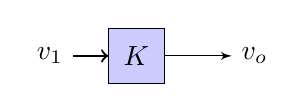
\begin{tikzpicture}[node distance=1.5cm,auto,>=latex']
		 \tikzstyle{int}=[draw, fill=blue!20, minimum size=2em]
		 \tikzstyle{init} = [pin edge={to-,thick,black}]
		 \node [int, pin={[init]left:$v_1$}] (a) {$K$};
		 \node (end) [right of=a, node distance=1.5cm]{$v_o$};
		 \draw[->] (a) -- (end) ;
		 %\draw[->] (c) edge node {$p$} (end) ;
		 \end{tikzpicture}  &
		  $ K_1 = \dfrac{Z_1+Z_2}{Z_2} $ 
		  \\ 
\begin{circuitikz}[american voltages,scale =0.8] \draw (0,0) node[op amp](amp9){}
	(amp9.out) to[short] (2,0) node[right](target) {}
	(2,1.5)  to[short,*-] (2,0)
	(2,1.5) to [short, -o] (2.5,1.5) node[right](end){$v_o$}
	(-2,1.5) to [R, l^= $Z_2$] (1,1.5) -- (1,1.5)
	(1,1.5) -- (2,1.5)
	(-2,1.5)to[short, *-](-2,0.60)
	(-2,0.60)to[short](amp9.-)
	(amp9.+) to[short] (-2,-0.6)
	(-2,1.5) to [R, l_= $Z_1$,-o] (-4,1.5) -- (-4,1.5) node[left](v1){$v_1$}
	(-2,-0.6) node[ground]{}
	node[below of = target,label={[align=right]Inverter}, xshift= -0.5cm, yshift = -0.1cm]{};
\end{circuitikz}
&

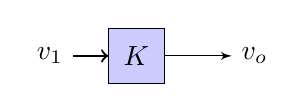
\begin{tikzpicture}[node distance=1.5cm,auto,>=latex']
\tikzstyle{int}=[draw, fill=blue!20, minimum size=2em]
\tikzstyle{init} = [pin edge={to-,thick,black}]
\node [int, pin={[init]left:$v_1$}] (a) {$K$};
\node (end) [right of=a, node distance=1.5cm]{$v_o$};
\draw[->] (a) -- (end) ;
%\draw[->] (c) edge node {$p$} (end) ;
\end{tikzpicture}
& 

$ K = -\dfrac{Z_2}{Z_1} $
\\ 

\begin{circuitikz}[american voltages,scale =0.8] \draw (0,0) node[op amp](amp8){}
	(amp8.out) to[short] (2,0) node[right](target) {}
	(2,1.5)  to[short,*-] (2,0)
	(2,1.5) to [short, -o] (2.5,1.5) node[right](end){$v_o$}
	(-2,1.5) to [R, l^= $Z_F$] (1,1.5) -- (1,1.5)
	(1,1.5) -- (2,1.5)
	(-2,1.5)to[short, *-](-2,0.60)
	(-2,0.60)to[short](amp8.-)
	(amp8.+) to[short] (-2,-0.6)
	(-2,1.5) to [R, l_= $Z_1$,-o] (-4,1.5) -- (-4,1.5) node[left](v1){$v_1$}
	(-2.25,0.6) to [R, l^= $Z_2$,-o] (-4,0.6) -- (-4,0.6) node[left](v2){$v_2$}
		(-2.25,0.6) -- (-2,1.5)
	(-2,-0.6) node[ground]{}
	node[below of = target,label={[align=right]Inverting\\Summer}, xshift= -0.5cm, yshift = -0.4cm]{};
\end{circuitikz}
&

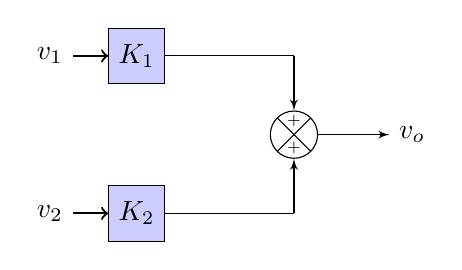
\begin{tikzpicture}[node distance=2cm,auto,>=latex']
	\tikzstyle{int}=[draw, fill=blue!20, minimum size=2em]
	\tikzstyle{init} = [pin edge={to-,thick,black}]
	(0,0) \node [int, pin={[init]left:$v_1$}] (a) {$K_1$};
	\node [int, pin={[init]left:$v_2$},below of=a] (b) {$K_2$};
	\node[draw,circle,add={+}{}{+}{},right of =a, yshift=-1cm](mixer){}; 
	\node (end) [right of=mixer, node distance=1.5cm]{$v_o$};
	\node [coordinate,right of =a](a2){};
	\node [coordinate,right of =b](b2){};
	%\node (end) [right of=a, node distance=1.5cm]{$v_o$};
	\draw[->] (mixer) -- (end) ;
	\draw[-] (a) -- (a2) ;
	\draw[-] (b) -- (b2) ;
	\draw[->] (a2) -- (mixer) ;
	\draw[->] (b2) -- (mixer) ;
\end{tikzpicture}
& 

$ K_1 = -\dfrac{Z_F}{Z_1} $
$	K_2 = -\dfrac{Z_F}{Z_2} $


 
 \\ 

 \begin{circuitikz}[american voltages,scale =0.8] \draw (0,0) node[op amp](amp7){}
 	(amp7.out) to[short] (2,0) node[right](target) {}
 	(2,1.5)  to[short,*-] (2,0)
 	(2,1.5) to [short, -o] (2.5,1.5) node[right](end){$v_o$}
 	(-2,1.5) to [R, l^= $Z_2$] (1,1.5) -- (1,1.5)
 	(1,1.5) -- (2,1.5)
 	(-2,1.5)to[short, *-](-2,0.60)
 	(-2,0.60)to[short](amp7.-)
 	(amp7.+) to[short] (-2,-0.6)
 	(-2,1.5) to [R, l_= $Z_1$,-o] (-4,1.5) -- (-4,1.5) node[left](v1){$v_1$}
 	(-2.25,-0.6) to [R, l^= $Z_3$,-o] (-4,-0.6) -- (-4,-0.6) node[left](v2){$v_2$}
 	(-2.25,-0.6) -- (-2,-0.6)
 	(-2,-0.6) to [R, l^= $Z_4$,*-] (-2, -2.25)node[ground]{}
 	node[below of = target,label={[align=right]Subtractor}, xshift= -0.5cm, yshift = -0.5cm]{};
 \end{circuitikz}
 &

 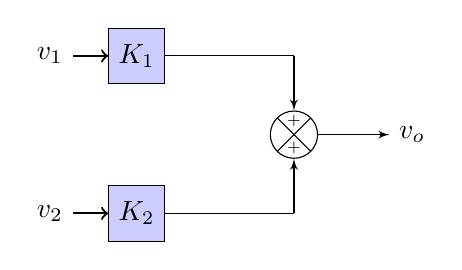
\begin{tikzpicture}[node distance=2cm,auto,>=latex']
 \tikzstyle{int}=[draw, fill=blue!20, minimum size=2em]
 \tikzstyle{init} = [pin edge={to-,thick,black}]
 (0,0) \node [int, pin={[init]left:$v_1$}] (a) {$K_1$};
 \node [int, pin={[init]left:$v_2$},below of=a] (b) {$K_2$};
 \node[draw,circle,add={+}{}{+}{},right of =a, yshift=-1cm](mixer){}; 
 \node (end) [right of=mixer, node distance=1.5cm]{$v_o$};
 \node [coordinate,right of =a](a2){};
 \node [coordinate,right of =b](b2){};
 %\node (end) [right of=a, node distance=1.5cm]{$v_o$};
 \draw[->] (mixer) -- (end) ;
 \draw[-] (a) -- (a2) ;
 \draw[-] (b) -- (b2) ;
 \draw[->] (a2) -- (mixer) ;
 \draw[->] (b2) -- (mixer) ;
 \end{tikzpicture}
 & 
 
 $ K_1 = -\dfrac{Z_2}{Z_1} $
 $	K_2 = \left(\dfrac{Z_1+Z_2}{Z_1} \right) \left(\dfrac{Z_4}{Z_3+Z_4} \right)$
 
 \\ 

  \begin{circuitikz}[american voltages,scale =0.8] \draw (0,0) node[op amp](amp5){}
  	(amp5.out) to[short] (2,0) node[right](target) {}
  	(2,1.5)  to[short,*-] (2,0)
  	(2,1.5) to [short, -o] (2.5,1.5) node[right](end){$v_o$}
  	(-2,1.5) to [C, l^= $C$] (1,1.5) -- (1,1.5)
  	(1,1.5) -- (2,1.5)
  	(-2,1.5)to[short, *-](-2,0.60)
  	(-2,0.60)to[short](amp5.-)
  	(amp5.+) to[short] (-2,-0.6)
  	(-2,1.5) to [R, l_= $R$,-o] (-4,1.5) -- (-4,1.5) node[left](v1){$v_1$}
  	(-2,-0.6) node[ground]{}
  	node[below of = target,label={[align=right]Integrator}, xshift= -0.5cm, yshift = -0.35cm]{};
  \end{circuitikz}
  &

  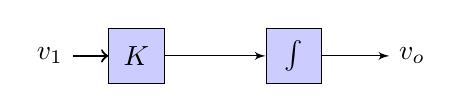
\begin{tikzpicture}[node distance=2cm,auto,>=latex']
  \tikzstyle{int}=[draw, fill=blue!20, minimum size=2em]
  \tikzstyle{init} = [pin edge={to-,thick,black}]
  (0,0) \node [int, pin={[init]left:$v_1$}] (a2) {$K$};
  \node [int,right of=a2] (b2) {$\int$};
  \draw [->] (a2) to (b2);
  \node(end2) [right of=b2, node distance=1.5cm] {$v_o$};
  \draw [->] (b2) to (end2);

%  \draw[->]b2 -- end2;
  \end{tikzpicture}
  & 
  
  $ K = -\dfrac{1}{RC} $
  \\ 

  \begin{circuitikz}[american voltages,scale =0.8] \draw (0,0) node[op amp](amp4){}
  	(amp4.out) to[short] (2,0) node[right](target) {}
  	(2,1.5)  to[short,*-] (2,0)
  	(2,1.5) to [short, -o] (2.5,1.5) node[right](end){$v_o$}
  	(-2,1.5) to [R, l^= $R$] (1,1.5) -- (1,1.5)
  	(1,1.5) -- (2,1.5)
  	(-2,1.5)to[short, *-](-2,0.60)
  	(-2,0.60)to[short](amp4.-)
  	(amp4.+) to[short] (-2,-0.6)
  	(-2,1.5) to [C, l_= $C$,-o] (-4,1.5) -- (-4,1.5) node[left](v1){$v_1$}
  	(-2,-0.6) node[ground]{}
  	node[below of = target,label={[align=right]Differentiator}, xshift= -0.5cm, yshift = -0.4cm]{};
  \end{circuitikz}
  &
    
  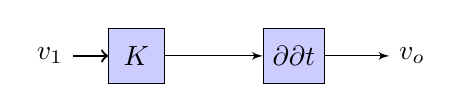
\begin{tikzpicture}[node distance=2cm,auto,>=latex']
  \tikzstyle{int}=[draw, fill=blue!20, minimum size=2em]
  \tikzstyle{init} = [pin edge={to-,thick,black}]
  (0,0) \node [int, pin={[init]left:$v_1$}] (a2) {$K$};
  \node [int,right of=a2] (b2) {${\partial}{ \partial t}$};
  \draw [->] (a2) to (b2);
  \node(end2) [right of=b2, node distance=1.5cm] {$v_o$};
  \draw [->] (b2) to (end2);
  
  %  \draw[->]b2 -- end2;
  \end{tikzpicture}
  & 
  
  $$ K = -RC $$ 
   \\ 

   \begin{circuitikz}[american voltages,scale =0.8] \draw (0,0) node[op amp,yscale=-1](amp2){}
   	(amp2.out) to[short] (1.5,1.5) node[right](target) {}
   	(2,1.5)  to[short,*-] (1.5,1.5)
   	(2,1.5) to [short, -o] (2.5,1.5) node[right](end){$v_o$}
   	(-2,1.5)to[short, -*](-2,0.60)
   	(-2,-0.60)to[short](amp2.-)
   	(amp2.+) to[short] (-2,0.6)
   	(-2,1.5) to [R, l_= $Z_1$,-o] (-4,1.5) -- (-4,1.5) node[left](v1){$v_1$}
   	(-2.25,0.6) to [R, l^= $Z_2$,-o] (-4,0.6) -- (-4,0.6) node[left](v2){$v_2$}
   	(2,1.5) to [R, l^= $R_A$,-*] (2,-0.25) -- (2,-0.25)
   	(2,-0.25) to [R, l^= $R_B$] (2,-2) -- (2,-2)
   	(-2.25,0.6) -- (-2,0.6)
   	(-2,-0.6) -- (-2,-2)
   	(-2,-2)	-- (1,-2)
   	(1,-2) -- (1, -0.25)
   	(1, -0.25) -- (2, -0.25)
   	(2,-2) node[ground]{}
   	node[below of = target,label={[align=right]Noninverting Summer}, xshift= -0.5cm, yshift = -3.25cm]{};
   \end{circuitikz}
   &

   \begin{tikzpicture}[node distance=2cm,auto,>=latex']
   \tikzstyle{int}=[draw, fill=blue!20, minimum size=2em]
   \tikzstyle{init} = [pin edge={to-,thick,black}]
   (0,0) \node [int, pin={[init]left:$v_1$}] (a) {$K_1$};
   \node [int, pin={[init]left:$v_2$},below of=a] (b) {$K_2$};
   \node [int,right of=mixer] (c) {$K_{AMP}$};
   \node[draw,circle,add={+}{}{+}{},right of =a, yshift=-1cm](mixer){}; 
   \node (end) [right of=c, node distance=1.5cm]{$v_o$};
   \node [coordinate,right of =a](a2){};
   \node [coordinate,right of =b](b2){};
   %\node (end) [right of=a, node distance=1.5cm]{$v_o$};
   \draw[->] (mixer) -- (c) ;
   \draw[->] (c) -- (end) ;
   \draw[-] (a) -- (a2) ;
   \draw[-] (b) -- (b2) ;
   \draw[->] (a2) -- (mixer) ;
   \draw[->] (b2) -- (mixer) ;
   \end{tikzpicture} 
   & 
   
   $ K_1 = -\dfrac{Z_2}{Z_1+Z_2} $
   $ K_2 = -\dfrac{Z_1}{Z_1+Z_2} $
   $ K_{AMP} = \dfrac{R_A+R_B}{R_B} $
  \\ 
%\tikzset{component/.style={draw,thick,circle,fill=white,minimum size =0.75cm,inner sep=0pt}}
\ctikzset{bipoles/length=0.8cm} 

\begin{circuitikz}[american voltages,scale =0.8] \draw (0,0) node[op amp](amp3){}
	(amp3.out) to[short, -o] (2,0) node[right](target) {$v_0$} 
	(1,0) to[short,*-] (1,1.5)
	(1,1.5) to[short] (-2,1.5)
	(-2,1.5)to[short](-2,0.60)
	(-2,0.60)to[short](amp3.-)
	(amp3.+) to[short, -o] (-2,-0.6)node[left] {$v_1$};
	\node[below of = target, xshift= -0.75cm, yshift = 0.25cm]{Follower};
\end{circuitikz}

& 
\tikzstyle{int}=[draw, fill=blue!20, minimum size=2em]
\tikzstyle{init} = [pin edge={to-,thick,black}]

\begin{tikzpicture}[node distance=1.5cm,auto,>=latex']
\node [int, pin={[init]left:$v_1$}] (a) {$K$};
\node (end) [right of=a, node distance=1.5cm]{$v_o$};
\draw[->] (a) -- (end) ;
%\draw[->] (c) edge node {$p$} (end) ;
\end{tikzpicture}&	K = 1	\\ 
		\bottomrule
\end{tabular}

\end{document}
